\chapter{TINJAUAN PUSTAKA}
\label{chap:tinjauanpustaka}

\section{Penelitian Terdahulu}
\label{sec:penelitianterdahulu}

\subsection{\emph{Analysis and Design of Calories Burning Calculation in Jogging Using Thresholding Based Accelerometer Sensor }(Okmuyura et al., 2019)}
\label{subsec:penelitian1}

Finanta Okmuyura, Noverta Effendi, Witri Ramadhani, dan Adlian Jefiza melakukan penelitian ini dengan membuat analisis dan desain untuk dapat memonitor pembakaran kalori saat jogging. Pada penelitian ini, dalam memonitor pembakaran kalori menggunakan sensor akselerometer yang dapat menghitung berdasarkan dari tekanan dari beban yang diterima untuk menghasilkan nilai \emph{threshold} untuk dikalkukasikan nantinya. Perhitungan kalori yang terbakar pada penelitian ini dengan menggunakan nilai jumlah langkah kaki, waktu dan berat pengguna untuk memberikan informasi pembakaran kalori dalam jogging.
  
\subsection{Sistem Prediksi Kalori Terbakar Pada Pesepeda Menggunakan \emph{Feedforward Neural Network} (Utami \& Ichwan, 2017)}
\label{subsec:penelitian2}

Dina Budhi Utami dan Muhammad Ichwan melakukan penelitian mengenai sistem prediksi kalori yang terbakar pada pesepeda menggunakan \emph{Feedforward Neural Network}. Penelitian ini melakukan prediksi berdasarkan detak jantung dan kecepatan kayuh saat bersepeda. Model prediksi kalori yang digunakan adalah \emph{Feedforward Neural Network} dengan arsitektur jaringan saraf tiruan terdiri dari 3 lapis. Hasil keluaran dari jaringan saraf tiruan adalah nilai prediksi kalori menggunakan pengujian 10000 data latih dengan memiliki tingkat kesalahan adalah 7\%.

\subsection{\emph{Estimating Physical Activity Intensity and Energy Expenditure Using Computer Vision on Videos} (Saponaro et al.,  2019)}
\label{subsec:penelitian3}

Pada tahun 2019, Philip Saponaro bersama Haoran Wei, Gregory Dominick dan Chandra Kambhamettu melakukan penelitian ini. Penelitian yang dilakukan mengenai perkirakan intensitas aktivitas fisik dan pengeluaran energi dengan menggunakan sistem visi komputer. Nilai perkiraan aktivitas fisik dan pengeluaran energi menggunakan faktor usia, jenis kelamin, kecepatan dan isyarat aktivitas. Data nilai usia dan jenis kelamin didapatkan dengan jaringan \emph{Deep Expectation} dan nilai aktivitas diperoleh dari perkiraan sudut sendi dan kecepatan gerak. Hasil yang didapat dengan akurasi nilai perkiraan aktivitas fisik sebesar 89,5\% dan perbedaan rata-rata pengeluaran energi sebesar 1,96 kCal/min.


\section{Kalori}
\label{sec:kalori}

Kalori merupakan pengukuran untuk menyatakan jumlah energi dalam makanan. Ketika makan dan minum, kita memberi kalori (energi) pada tubuh. Tubuh akan memakai kalori untuk bahan bakar aktivitas yang dilakukan. Banyaknya aktivitas yang dilakukan, maka banyak pula kalori (energi) yang dibutuhkan. Jumlah kalori dalam makanan dapat ditulis dalam satuan ‘kkal’ (kilokalori). Kalori adalah kebutuhan yang sangat penting bagi semua orang untuk kelangsungan hidupnya. Kalori merupakan hal utama sebagai penyokong tubuh dalam melakukan berbagai aktivitas (Inmawati N. D., 2016). 

Kebutuhan kalori bisa dihitung berdasarkan gender, umur, tinggi dan berat badan, komposisi tubuh, aktivitas, serta kondisi fisik seseorang. Kebutuhan kalori laki-laki berbeda dengan perempuan meskipun rentang umurnya sama. Jika kegiatan yang dilakukan membutuhkan aktivitas fisik yang lebih berat, maka kebutuhan akan asupan kalori harian meningkat. Mengetahui kebutuhan energi per hari bisa membantu menjaga kesehatan karena hal tersebut dapat mempengaruhi keseimbangan energi harian seseorang. Semakin banyak jenis makanan yang memiliki kandungan rendah kalori, atau masyarakat sering menyebutnya sebagai \emph{low fat}. Banyak sekali masyarakat yang tidak terakomodasi dengan baik perhatiannya akan kalori tersebut.

Tidak ada cara akurat untuk menghitung kalori. Beberapa faktor seperti berat badan, intensitas aktifitas, kondisi tubuh dan metabolisme. Aktivitas fisik akan membakar energi dalam tubuh sehingga jika asupan kalori ke dalam tubuh berlebihan dan tidak diimbangi dengan aktivitas fisik yang seimbang akan menyebabkan tubuh mengalami kegemukan. Semakin tua usia seseorang, kurang aktif bergerak menyebabkan massa otot dalam tubuh cenderung menurun dan kehilangan otot menyebabkan perlambatan tingkat pembakaran kalori dalam tubuh. Semakin bertambah usia dan dengan asupan kalori yang tetap, tubuh semakin sulit untuk membakar kalori yang masuk sehingga terjadi penumpukan energi didalam tubuh dan berdampak pada obesitas (Widiantini et al., 2013).


\section{Regresi Linear}
\label{sec:regresi}




Regresi linier merupakan satu cara prediksi yang menggunakan garis lurus untuk menggambarkan hubungan diantara dua variabel (atau lebih) (Kurniawan, 2008). Regresi linier merupakan salah satu metode statistika yang digunakan untuk membentuk model hubungan antara variabel terikat (dependen; respon; Y) dengan satu atau lebih variabel bebas (independen, prediktor, X).  Apabila banyaknya variabel bebas hanya ada satu, disebut sebagai regresi linier sederhana, sedangkan apabila terdapat lebih dari 1 variabel bebas, disebut sebagai regresi linier berganda. Analisis regresi merupakan metode statistika yang banyak digunakan dalam penelitian. Istilah regresi pertama kali diperkenalkan oleh Sir Francis Galton pada tahun 1986.  Secara umum, analisis regresi adalah kajian terhadap hubungan satu variabel yang disebut sebagai variabel yang diterangkan dengan satu atau dua variabel yang menerangkan (Syilfi \& Ispriyanti, 2012). Variabel yang diterangkan selanjutnya disebut sebagai variabel respon, sedangkan variabel yang menerangkan biasa disebut variabel bebas. 

Terdapat 3 kegunaan dalam penggunaan regresi liner, diantaranya yaitu untuk tujuan deskripsi dari fenomena data atau kasus yang sedang diteliti, untuk tujuan kontrol, serta untuk tujuan prediksi. Regresi mampu mendeskripsikan fenomena data melalui terbentuknya suatu model hubungan yang bersifatnya numerik. Regresi juga dapat digunakan untuk melakukan pengendalian (kontrol) terhadap suatu kasus atau hal-hal yang sedang diamati melalui penggunaan model regresi yang diperoleh. Selain itu, model regresi juga dapat dimanfaatkan untuk melakukan prediksi untuk variabel terikat. Namun yang perlu diingat, prediksi di dalam konsep regresi hanya boleh dilakukan di dalam rentang data dari variabel-variabel bebas yang digunakan untuk membentuk model regresi tersebut. Misal, suatu model regresi diperoleh dengan mempergunakan data variabel bebas yang memiliki rentang antara 5 s.d. 25, maka prediksi hanya boleh dilakukan bila suatu nilai yang digunakan sebagai input untuk variabel X berada di dalam rentang tersebut. Konsep ini disebut sebagai interpolasi (Sulardi et al., 2017).

Data untuk variabel independen X pada regresi linier bisa merupakan data pengamatan yang tidak ditetapkan sebelumnya oleh peneliti (\emph{obsevational data}) maupun data yang telah ditetapkan (dikontrol) oleh peneliti sebelumnya (\emph{experimental or fixed data}). Perbedaannya adalah bahwa dengan menggunakan \emph{fixed data}, informasi yang diperoleh lebih kuat dalam menjelaskan hubungan sebab akibat antara variabel X dan variabel Y. Sedangkan, pada \emph{observational data}, informasi yang diperoleh belum tentu merupakan hubungan sebab-akibat. Untuk \emph{fixed data}, peneliti sebelumnya telah memiliki beberapa nilai variabel X yang ingin diteliti. Sedangkan, pada \emph{observational data}, variabel X yang diamati bisa berapa saja, tergantung keadaan di lapangan. Biasanya, \emph{fixed data} diperoleh dari percobaan laboratorium, dan \emph{observational data} diperoleh dengan menggunakan kuesioner.


\section{Deteksi Gestur Tubuh}
\label{sec:deteksigesturtubuh}

Deteksi gestur tubuh atau yang dapat disebut \emph{body pose recognition} merupakan teknologi yang mampu membaca gerak pose tubuh kemudian menjadikan proses yang diinginkan oleh peneliti. Deteksi gestur ini merupakan topik dalam \emph{computer science} yang memiliki tujuan agar komputer dapat memahami gerakan manusia yang berasal dari postur tubuh.


\section{\emph{Deep Learning}}
\label{sec:deeplearning}

\emph{Deep learning} adalah salah satu bidang \emph{machine learning} yang memanfaatkan banyak \emph{layer} pengolahan informasi nonlinier untuk melakukan ekstraksi fitur, pengenalan pola, dan klasifikasi (Deng dan Yu, 2014). Menurut Goodfellow, dkk. (2016), \emph{Deep learning} adalah sebuah pendekatan dalam penyelesaian masalah pada sistem pembelajaran komputer yang menggunakan konsep hierarki. Konsep hierarki membuat komputer mampu mempelajari konsep yang kompleks dengan menggabungkan dari konsep-konsep yang lebih sederhana. Jika digambarkan sebuah graf bagaimana konsep tersebut dibangun di atas konsep yang lain, graf ini akan dalam dengan banyak layer, hal tersebut menjadi alasan disebut sebagai \emph{Deep learning} (pembelajaran mendalam).

\emph{Deep learning} terdiri dari banyak lapisan (\emph{hidden layer}) dan membentuk tumpukan, lapisan tersebut adalah sebuah algoritma atau metode yang melakukan klasifikasi perintah yang diinput hingga menghasilkan \emph{output}. Metode \emph{deep learning} yang sedang berkembang salah satunya adalah \emph{Convolutional Neural Network}. Jaringan ini menggunakan masukan berupa gambar, kemudian akan melalui lapisan konvolusi dan diolah berdasarkan filter yang ditentukan, setiap lapisan ini menghasilkan pola dari beberapa bagian citra yang memudahkan proses klasifikasi (Danukusumo, 2017).

Metode \emph{Deep Learning} yang saat ini memiliki hasil paling signifikan dalam pengenalan citra adalah \emph{Convolutional Neural Network} (CNN) (Nugroho et al., 2020). Hal tersebut dikarenakan CNN berusaha meniru sistem pengenalan citra pada visual cortex manusia sehingga memiliki kemampuan mengolah informasi citra. Namun, CNN seperti metode \emph{Deep Learning} lainnya, memiliki kelemahan yaitu proses pelatihan model yang lama. Dengan perkembangan perangkat keras, hal tersebut dapat diatasi menggunakan teknologi \emph{General Purpose Graphical Processing Unit} (GPGPU). CNN dirancang khusus untuk pengenalan dan klasifikasi gambar. CNN memiliki beberapa lapisan (\emph{layer}) yang mengekstrak informasi dari gambar dan menentukan klasifikasi dari gambar berupa skor klasifikasi.


\section{\emph{Convolutional Neural Network}}
\label{sec:cnn}

\emph{Convolutional Neural Network} (CNN) adalah salah satu jenis perhitungan \emph{neural network} yang sering digunakan pada pengolahan citra untuk mendeteksi dan mengenali objek pada sebuah \emph{image} (Mehindra, 2020). CNN berupa jaringan saraf yang dikhusukan untuk memproses data yang memiliki grid. CNN juga dapat diartikan sebagai kombinasi dari jaringan syaraf tiruan dan metode \emph{deep learning} (Fonda, 2020). CNN terdiri dari satu atau lebih lapisan konvolutional, seringnya dengan suatu lapisan \emph{dubsampling} yang diikuti oleh satu atau lebih lapisan yang terhubung penuh sebagai standar jaringan syaraf.

Arsitektur dari CNN juga terbagi menjadi 2 bagian besar yaitu \emph{Feature Extraction Layer} dan \emph{Fully-Connected Layer} (MLP). Sebuah CNN terdiri dari beberapa layer. Berdasarkan aristektur LeNet5, terdapat empat macam layer utama pada sebuah CNN yaitu \emph{Convolution Layer, Pooling Layer, Subsampling Layer,} dan \emph{Fully Connected Layer} (Eka Putra, 2016).

Pada CNN, data yang dipropagasikan oleh jaringan adalah data dua dimensi, sehingga operasi linear dan parameter bobot pada CNN berbeda. Pada CNN operasi linear menggunakan operasi konvolusi, sedangkan bobot tidak lagi satu dimensi saja, namun berbentuk empat dimensi yang merupakan kumpulan kernel konvolusi. Karena sifat proses konvolusi, maka CNN hanya dapat digunakan pada data yang memiliki struktur dua dimensi seperti citra dan suara.

Sebagai contoh adalah berupa citra dua dimensi. Nama konvolusi sendiri merupakan operasi aljabar linear yang mengkalikan matriks dari filter pada citra yang akan di proses. Proses ini disebut lapisan konvolusi dan merupakan salah satu jenis dari banyak lapisan bisa dimiliki dalam satu jaringan. Lapisan konvolusi merupakan lapisan utama yang paling penting untuk digunakan. Jenis lapisan lain yang biasa digunakan adalah \emph{Pooling Layer}, yakni lapisan yang digunakan untuk mengambil nilai maksimal atau nilai rata-rata dari bagian-bagian piksel pada citra. Setiap lapisan input yang dimasukkan memiliki volume yang berbeda da mewakili dengan kedalaman, tinggi dan lebar. Setiap besaran yang didapatkan tergantung dari hasil filtrasi dari lapisan sebelumnya dan juga banyak filter yang digunakan. Model jaringan seperti ini sudah terbukti sangat ampuh dalam menangani permasalahan klasifikasi citra. 


\section{Mediapipe}
\label{sec:mediapipe}

Mediapipe adalah kerangka kerja yang terutama digunakan untuk menghasilkan audio atau video Dengan bantuan \emph{framework} MediaPipe, \emph{pipeline Machine Learning} dapat dibuat untuk instance model inferensi seperti TensorFlow, TFLite, dan juga untuk fungsi pemrosesan media, bahkan tidak memerlukan GPU untuk menjalankan eksperimen dengan MediaPipe, karena grafik dan CPU terintegrasi saat ini bekerja dengan baik untuk solusi ini. Logikanya, FPS jauh lebih rendah daripada penggunaan GPU, tampak pada Gambar \ref{fig:mediapipe}.

\begin{figure}[H]
  \centering
  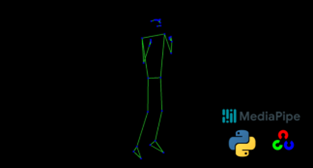
\includegraphics[scale=1]{gambar/mediapipe.png}
  \caption{Mediapipe untuk Pose Estimation.}
  \label{fig:mediapipe}
\end{figure}
